 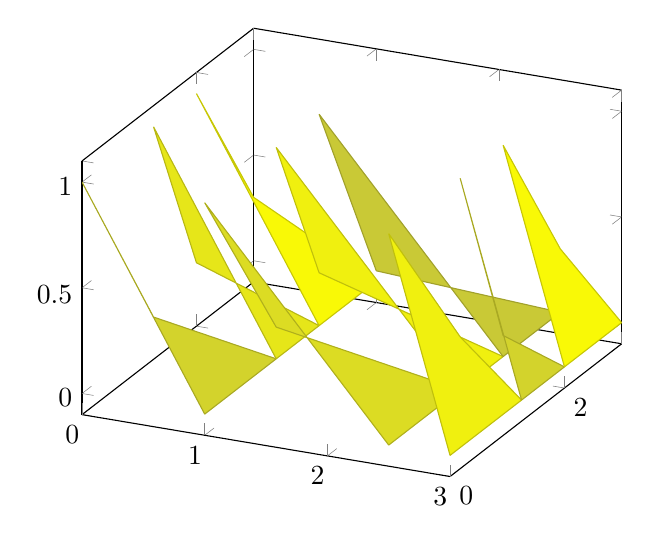
\begin{tikzpicture}
        \begin{axis}%[
            view={0}{90},
            xlabel=quantity of wine,
            ylabel=grape quality,
            colorbar,
            colormap/blackwhite
            ]
			%\addplot[color=red]{exp(x)};
            \addplot3[patch,shader=faceted,patch type=rectangle] coordinates {(0,0,   1) (1,0,   0) (1,1.25,0) (0,1.25,0.1)};
            \addplot3[patch,shader=faceted,patch type=rectangle] coordinates {(0,1.25,1) (1,1.25,0) (1,2,   0) (0,2,   0.2)};
            \addplot3[patch,shader=faceted,patch type=rectangle] coordinates {(0,2,   1) (1,2,   0) (1,3,   0) (0,3,   0.3)};
            \addplot3[patch,shader=faceted,patch type=rectangle] coordinates {(1,0,   1) (2.5,0,   0) (2.5,1.25,0) (1,1.25,0.15)};
            \addplot3[patch,shader=faceted,patch type=rectangle] coordinates {(1,1.25,1) (2.5,1.25,0) (2.5,2,   0) (1,2,   0.25)};
            \addplot3[patch,shader=faceted,patch type=rectangle] coordinates {(1,2,   1) (2.5,2,   0) (2.5,3,   0) (1,3,   0.05)};
            \addplot3[patch,shader=faceted,patch type=rectangle] coordinates {(2.5,0,   1) (3,0,   0) (3,1.25,0) (2.5,1.25,0.25)};
            \addplot3[patch,shader=faceted,patch type=rectangle] coordinates {(2.5,1.25,1) (3,1.25,0) (3,2,   0) (2.5,2,   0.1)};
            \addplot3[patch,shader=faceted,patch type=rectangle] coordinates {(2.5,2,   1) (3,2,   0) (3,3,   0) (2.5,3,   0.3)};
        \end{axis}
\end{tikzpicture}